\section{Inledning}
	
	%Vadå ramverk för agil uppskalning
	Detta arbete jämför olika ramverk för uppskalning av agil programutveckling. Dessa ger metoder och principer för att applicera mer traditionella agila metoder på större projekt och grupper.
	
	%agila metoder
	Agil programutveckling är i sig ett iterativt och inkrementellt sätt att utveckla programvara.
	
	%meta
	Detta arbete är indelat i fyra huvudkapitel. Inledningen utgör i sin helhet det första kapitilet.
	I andra kapitlet behandlas bakgrunden till själva frågeställningen. Tekniska definitioner för Agil utveckling, dess skalning samt de olika ramverken för det presenteras. 
	Det tredje kapitlet formulerar syftet med arbetet samt ämnets avgränsningar. Materialet och vilka metoder som används presenteras även i tredje kapitlet.
	
	Sista kapitlet behandlar själva reslutatet av arbetet och vilka slutsatser som dras av det.
	
\newpage
\section{Bakgund} 	
	
	%TODO: Teoretisk bakgrund och genomgång av problemuppläggningen
	
	I detta stycke behandlas den tekniska bakgrunden till arbetet. All bakgrundskunskap förutsatt av läsaren presenteras här.
	
	\subsection{Agil utveckling}
	
	Agil utveckling är en metod, eller en samling principer, för programutveckling. Principerna bygger på att bryta ner en stor helhet i små mindre självständiga delar, som man sedan utvecklar i skilda etapper, ofta kallade Sprinter.
	Mellan varje sprint finns möjlighet för kunden och utvecklarna att komma med förändringsförslag och kommentera förra sprintens resultat. Varje sprint ska producera en fungerande helhet som läggs till huvudprodukten. Centrala begrepp och principer inom agil programutveckling är transparens, flexibilitet samt inkrementell och iterativ utveckling. Man värdesätter flexibilitet och kommunkation med kunden över en noggrannt specifierad process som sedan följs. \cite{agile_manifesto}
	
	\subsection{Skalning av agil utveckling}
	%Vad är skalning, hur får mad det att fungera.
	Agila metoder används traditionellt i 
	
	
	\subsection{Large-Scale Scrum}
	
	
	
	
	Några grundläggande LeSS principer: \cite{less_principles}
	
	\begin{itemize}
		\setlength{\itemsep}{1pt}
		\item LeSS är Scrum - använd Scrum-principer oförändrat i ett större sammanhang			
		\item Transparens
		\item ''\textbf{More} with \textbf{LeSS}'' dvs. \textbf{Mera} med \textbf{mindre}
			\begin{itemize}
				\item \textbf{Mer} inlärning med \textbf{mindre} definierade processer
				\item \textbf{Mer} värde med \textbf{mindre} omkostnader
				\item \textbf{Mer} ägarskap och syfte med \textbf{mindre} huvudroller och specialgrupper
			\end{itemize}
		\item Kundcentrerat
		\item Systemtänkande
	\end{itemize}
	
	\subsection{Scaled Agile Framework}
	
	
	Några grundläggande SAFe principer: \cite{safe_principles}
	\begin{itemize}
		\item Ekonomisk synpunkt
		\item Systemtänkande
		\item Förvänta förändring - bevara möjligheter
		\item Bygg inkrementellt med snabba inlärningsintervall
		\item Basera milstolpar på en objektiv värdering av ett fungerande system
		\item Visualisera och begränsa pågående arbete
	\end{itemize}
	
	
	\subsection{Disciplined Agile}
	
	
	Några grundläggande DAD principer: \cite{dad_principles}
		
	\newpage

\section{Syfte, avgränsningar, material och metoder}
	
	
	\subsection{Syfte}
	%TODO: Syftet med arbetet
	
	Syftet med arbetet är att klargöra vilka skillnader det finns mellan olika ramverk för skalning av agil utveckling. Tekniska skillnader i användningen och definitionerna av ramverken pekas ut och analyseras.
	Tyngdpunkten ligger på att redogöra för vilka situationer olika ramverk lämpar sig bättre än andra, och att ställa ramverkens styrkor och svagheter mot varandra. \newline
	En central forskningsfråga är att utreda på basis av vilka kriterier ett företag väljer att använda sig av ett visst ramverk.
	
	
	
	
	\subsection{Avgränsning}
	%TODO: Avgränsa arbetet
	
	Ramverken som jämförs i detta arbete är begränsade till Large Scale Scrum (LeSS), Scaled Agile Framework (SAFe) samt Disciplined Agile Delivery (DAD).
	
	Av dessa tre är LeSS och SAFe mer etablerade och har används i relativt stor utsträckning. DAD är ett nyare ramverk, och har således inte uppnått samma användninsnivå som de andra. DAD fungerar dock som en bra jämförelsepunkt i arbetet i och med att det till skillnad från ett flertal andra ramverk styrks av omfattande dokumentation som till sin kvalitét är fullt jämförbar med den tillgänglig för Less och SAFe. \cite{ask_matrix}
	
	
	\subsection{Material och metoder}
	%TODO: Beskriv arbtessättet, speciellt för informationssökningens del
	I arbetet andänds huvudsakligen två olika sorters material.
	
	Jämförelsen av ramverkens tekniska speficikationer och principer sker på basis av tillgänglig dokumentation. Böcker och tekniska speficikationer används.
	\linebreak
	
	Ramverkens styrkor, svagheter och användingsmöjligheter jämförs primärt på basis av fallstudier gjorde av företag som använt sig av ramverken i praktiken.
	
	%todo Fräsig matris/statistik på fallstudier per ramverk( och kvalitén på dessa?)
	
	
	Arbetets analys och slutsatser är starkt bundna av tillgången till material och på kvalitén av det tillgängliga materialet. Speciellt fallstudier kan vara vinklade i något visst ramverks fördel, eftersom företag inte vill rapportera dåliga resultat eller misslyckade projekt. Konsulter vill ofta inte heller erkänna att de använt sig av ifrågasättbara metoder.
	
	
	Tabell över tillgängligt material för de olika ramverken:

	\begin{center}
	\begin{tabular}{ >{\bfseries}l | r | r | r }
		 	 						& Böcker & Artiklar & Fallstudier 	\\ \hline
		Disciplined Agile Delivery 	& 1 	& 2			& 2 			\\ \hline
		Large Scale Scrum 			& 3 	& >10		& 21 			\\ \hline
		Scaled Agile Framework 		& 4 	& >10		& 27 			\\ 
	\end{tabular}
	\end{center}
	
	Källa: Ramverkens respektive hemsidor\cite{dad_web, less_web, safe_web}, samt sökningar i vetenskapliga databaser(via bl.a. Google Scholar) med ramverken som sökord.
	
	
	%Hemsidor:
	%http://www.disciplinedagiledelivery.com/
	%http://scaledagileframework.com/
	%http://less.works/
	
\newpage
\section{Resultat}
	
	%Behöver inspiration\\
		
	
	\subsection{Gemensamma egenskaper hos ramverken}
		
	
	\subsection{Användningsområden}

	Fallstudier sammanfattar hur implementationen av ramverket i företaget gått och framförallt vilket resultat man uppnått. Det framgår sällan vilken sorts förhandsarbete som gjorts, och vilka kriterier man satt ut innan man valde att använda sig av ett enskilt ramverk.
	För att således kunna dra någon form av slutsats gällande vilka orsaker företag har för att välja ramverk har företagen indelats enligt branch.
	Ramverk som favoriserats av en specifik branch kan antas vara väl mer lämpat för ett dylikt företag än de andra ramverk.

	%todo Sätt in Grafer på fallstudier, vilken sorts företag använder sig av respektive ramverk
	
	\begin{center}
		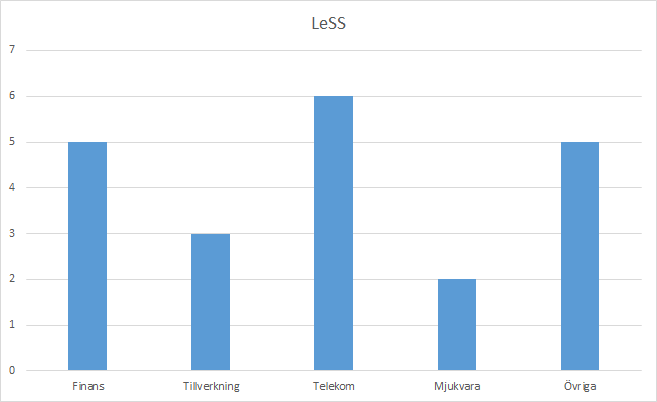
\includegraphics{Grafer/LeSS_brancher.png}
	\end{center}
	
	LeSS har en tyngdunkt på finans och telekombranchen.
		
	\begin{center}
		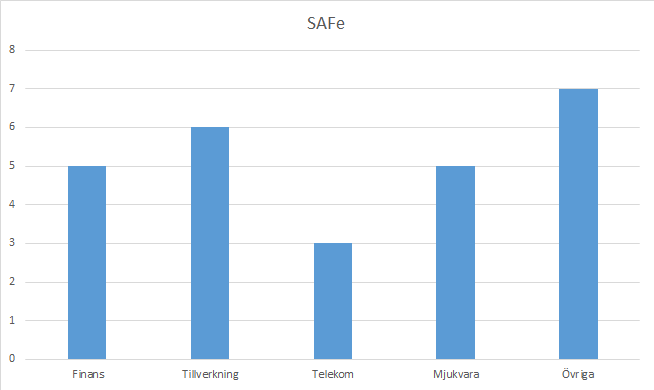
\includegraphics{Grafer/SAFe_brancher.png}
	\end{center}
	
	
	
	Finansbranchen är återkommande för de båda stora ramverken. Inom finans är det höga krav på säkerhet och kvalitét när det kommer till system. Dessutom finns det sällan ekonomiska hinder för projekt som är av tillräcklig storlek för att behöva tillämpa ett ramverk för uppskalning. 
	
	Märkbara skillnader 
	%todo diskutera varför skillnaderna uppstår, dvs telekom vs. tillverkning -> färdig struktur (löpande band etc) vs kaos
	
	
	\subsubsection{SAFe}
		
	
	\subsubsection{LeSS}
	
	\subsubsection{DAD}
	
	\subsection{Nämnvärda skillnader}